\chapter{Feature Extraction with Point Features}

\section{Overview}

To improve the estimate of the state and to get an idea of our environment, we need to understand the input of our exteroceptive sensors. As seen in chapter \ref{cha:Platform}, our robot is equipped with both a Camera and a LIDAR. In this chapter we try to use a simple algorithm based to detect fixed features in the environment. We then try to improve upon the algorithm by using our preexisting knowledge of the environment.  

\section{Feature Extraction Algorithm}

Consider an extremely clean environment. One which has only fixed features and they are all away from the wall. And the entire environment is within the range of the LIDAR. In such an environment the distance readings gradually increase and decrease all along the walls except when they encounter and obstacle or a \textit{feature}. This algorithm essentially looks for large jumps in the distance readings. One such arena is shown in figure \ref{fig:Simulated_1}. The gradual nature of the distance readings are more clearly seen when we plot the scan values as a function of the angle of the scan beam with respect to the robot as done in figure \ref{fig:Vrep_plot}.
\begin{figure}[h!]
    \centering
    \begin{subfigure}[b]{0.3\textwidth}
	    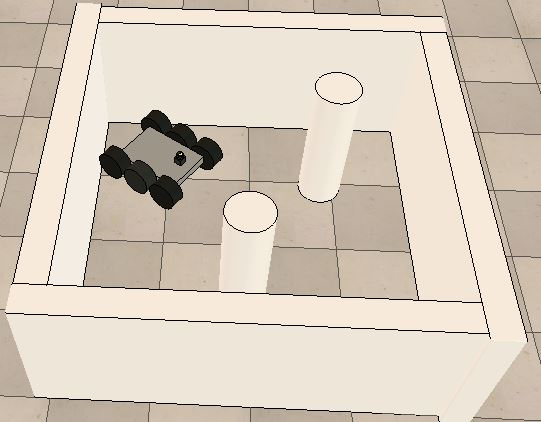
\includegraphics[width=\textwidth]{3d_vrep}
	    \caption{A simulated arena}
	    \label{fig:3d_vrep}
    \end{subfigure}
    \quad %add desired spacing between images, e. g. ~, \quad, \qquad, \hfill etc.
      %(or a blank line to force the subfigure onto a new line)
    \begin{subfigure}[b]{0.3\textwidth}
        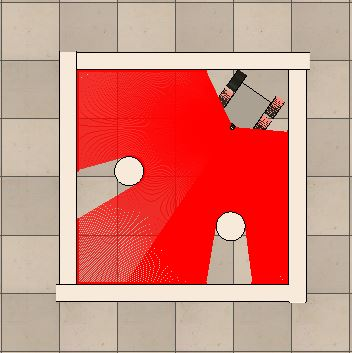
\includegraphics[width=\textwidth]{arena_vrep}
        \caption{Top view}
        \label{fig:arena_vrep}
    \end{subfigure}%
        \caption{Simulated Arena for LIDAR}
        \label{fig:Simulated_1}
\end{figure}

For the robot to detect the large jumps we differentiate the distance with respect to angles. As seen in figure \ref{fig:Vrep_cylinders} this will give a specific pattern each time a cylinder is present. A condition can then be designed in the following way. Each time the derivative is larger than a fixed threshold and is a negative number, a cylinder's beginning is found, and when a large positive value is encountered, it's end. Finding the mid point of these two readings we find the location of the cylinder as in figure \ref{fig:Vrep_cylinders}. 
\begin{figure}
        \centering

        \begin{subfigure}[b]{0.48\textwidth}
                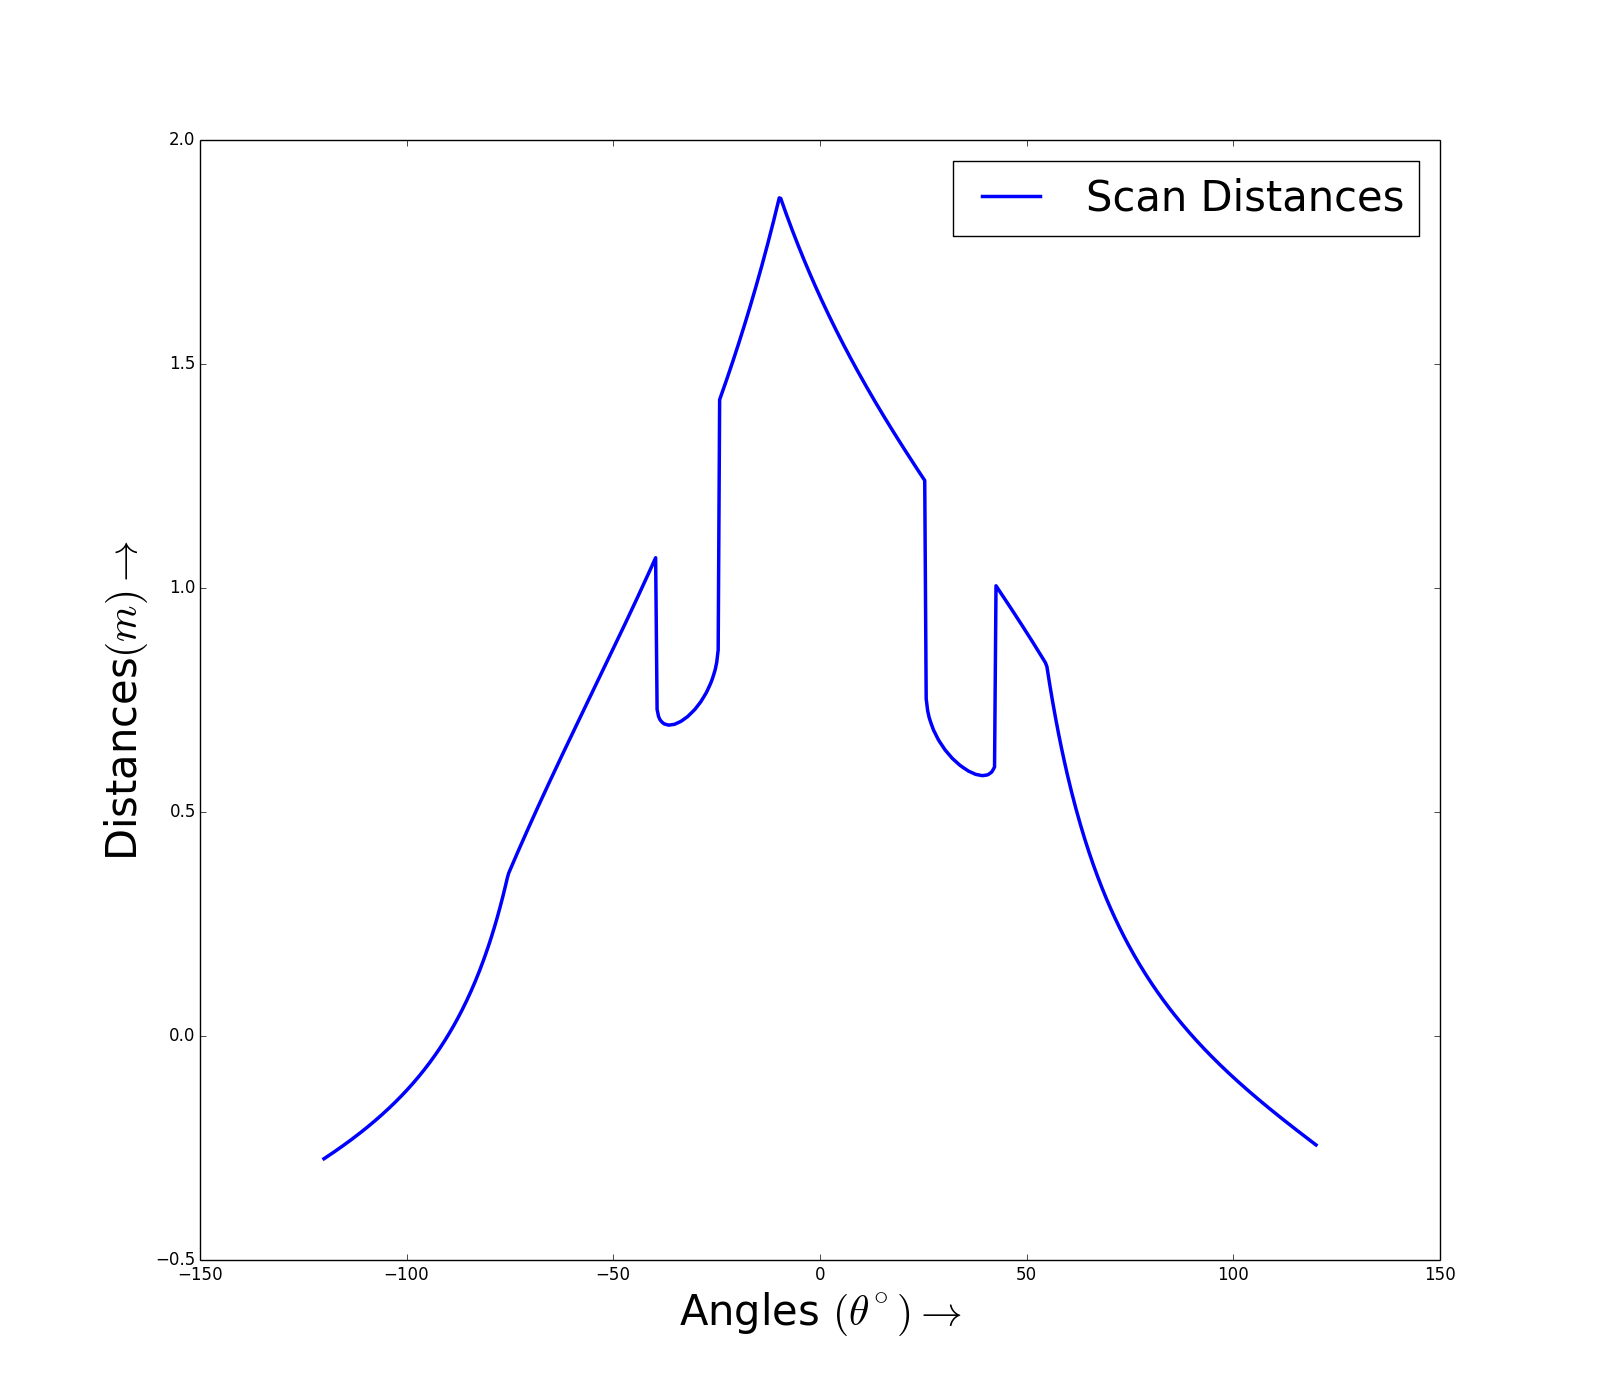
\includegraphics[width=\textwidth]{Vrep_plot}
                \caption{LIDAR scan}
                \label{fig:Vrep_plot}
        \end{subfigure}
        \quad %add desired spacing between images, e. g. ~, \quad, \qquad, \hfill etc.
          %(or a blank line to force the subfigure onto a new line)
%        \begin{subfigure}[b]{0.3\textwidth}
%                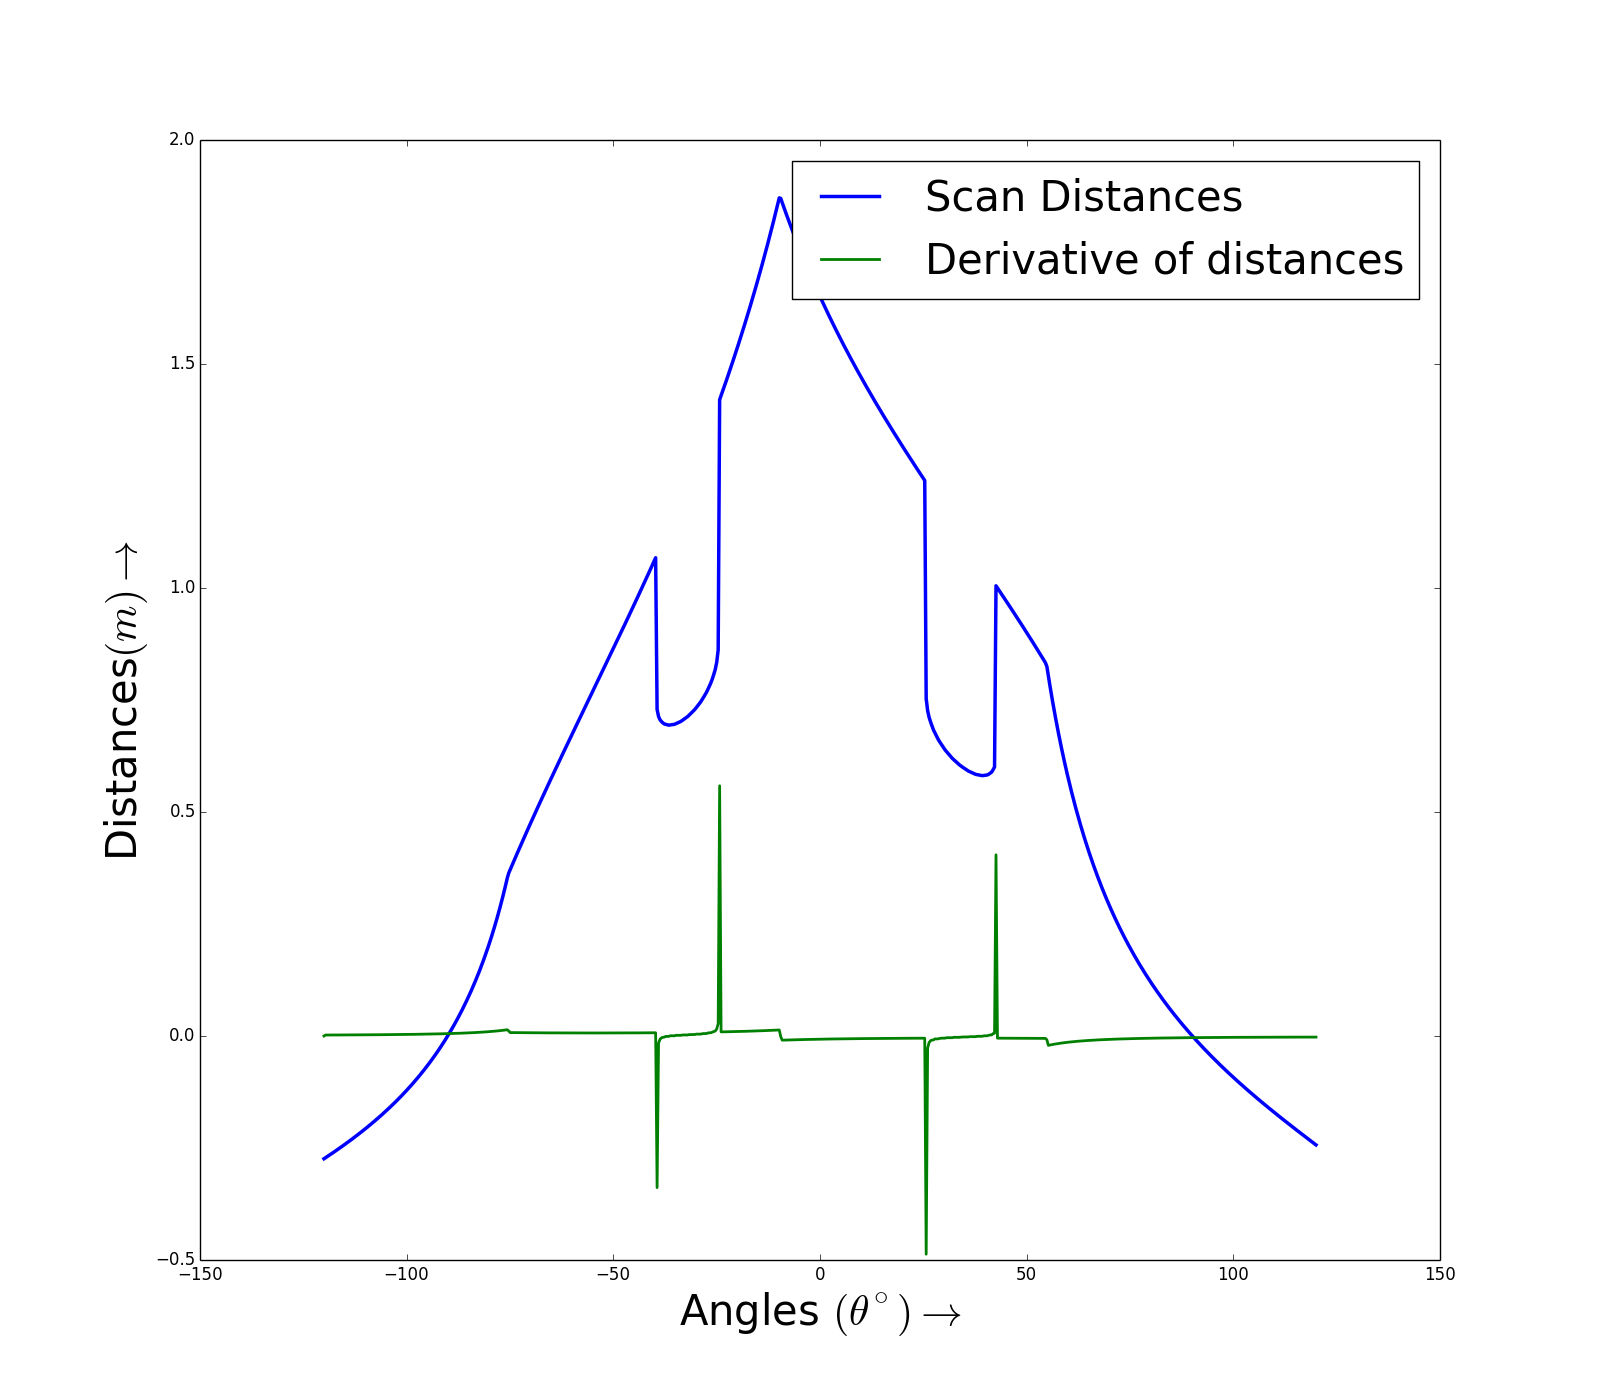
\includegraphics[width=\textwidth]{Vrep_derivative}
%                \caption{Derivative of scan}
%                \label{fig:Vrep_derivative}
%        \end{subfigure}%
        \quad %add desired spacing between images, e. g. ~, \quad, \qquad, \hfill etc.
          %(or a blank line to force the subfigure onto a new line)
        \begin{subfigure}[b]{0.48\textwidth}
                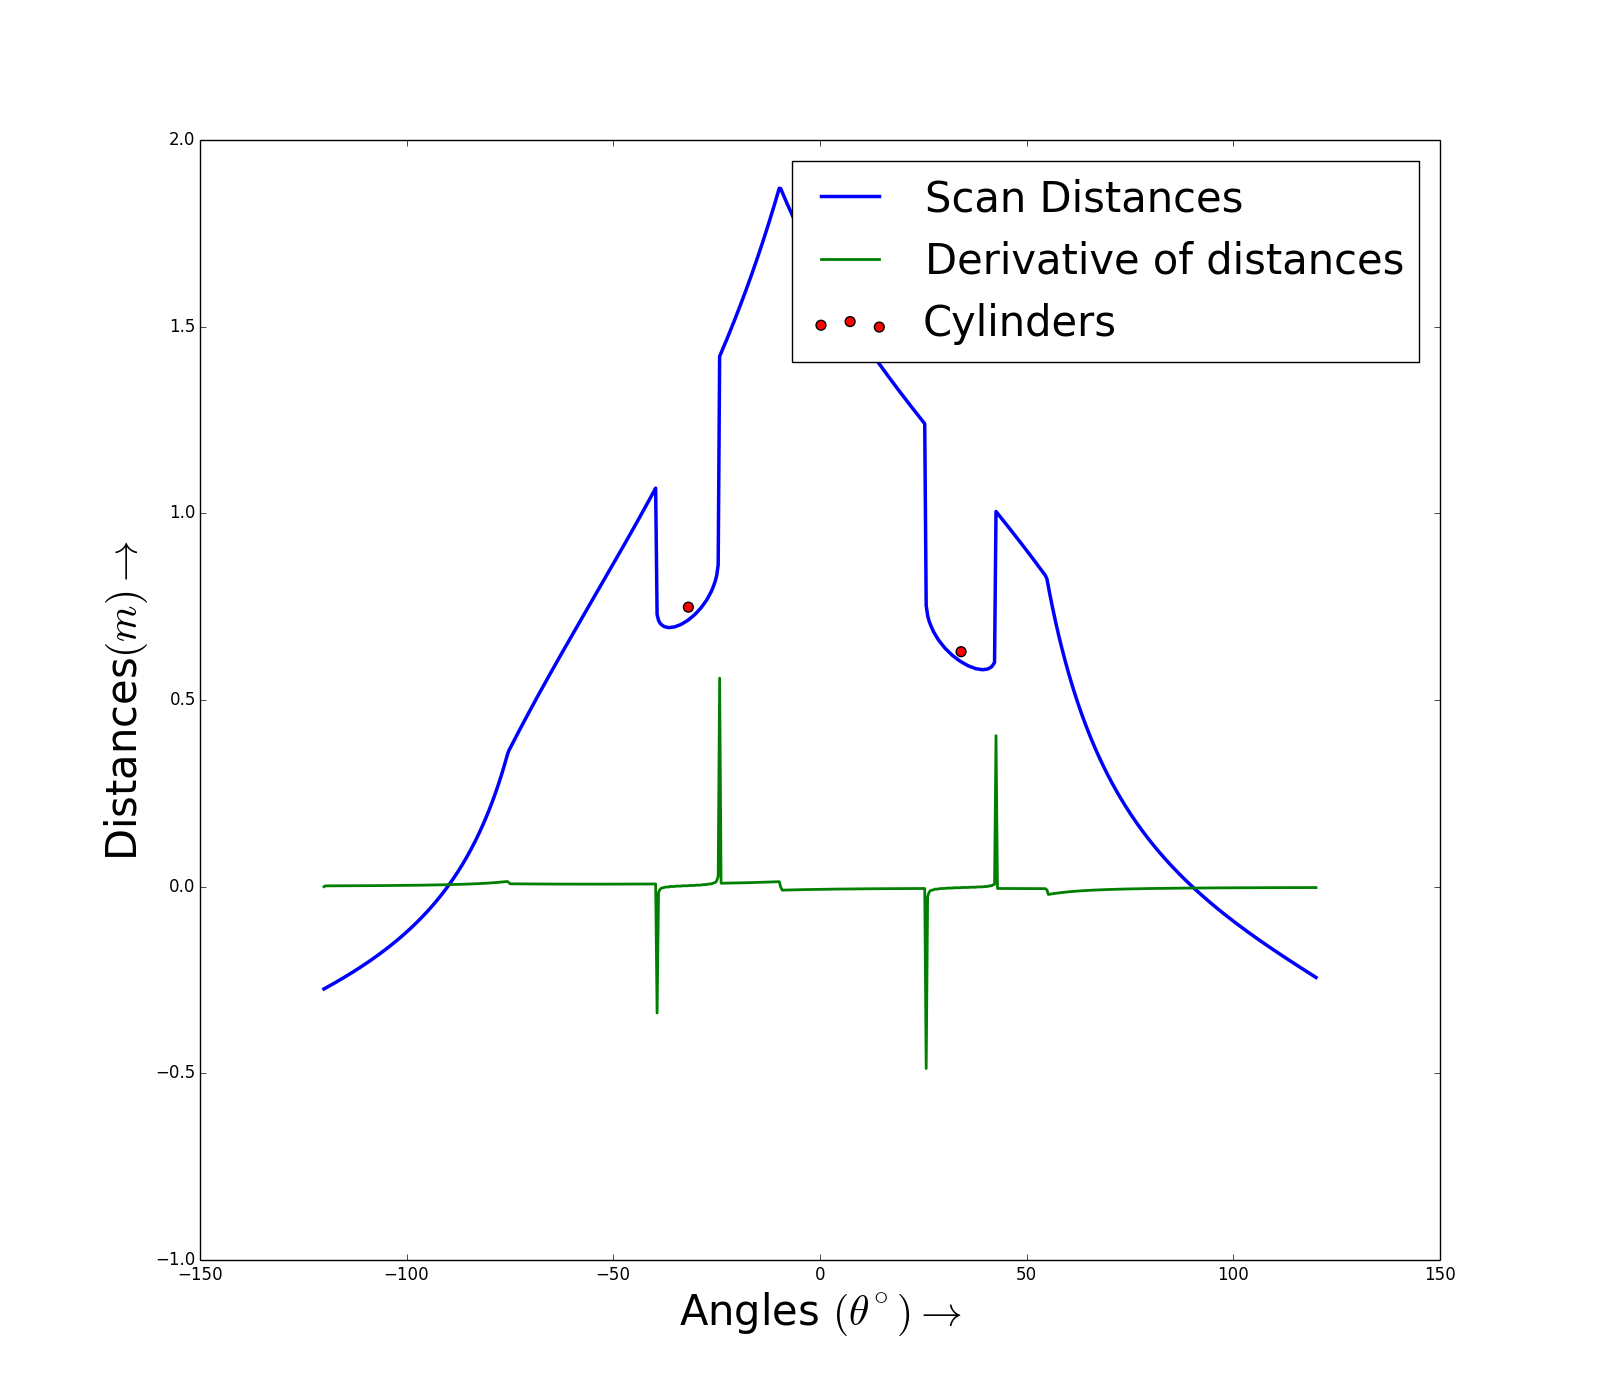
\includegraphics[width=\textwidth]{Vrep_cylinders}
                \caption{Detected cylinders}
                \label{fig:Vrep_cylinders}
        \end{subfigure}

        \caption{Differential based LIDAR feature detection}\label{fig:Simulated_2}
\end{figure}

It is apparent this method has a large number of drawbacks. The arena has to be fully within the range of the sensor, if not there will be breaks in the distance curve that will generate spurious landmarks. This drawback can be easily overcome by creating a zero order hold for those regions. Also any disturbances in the boundaries will also generate spurious landmarks. The threshold for the derivative is a very sensitive tuning parameter. If we set it too high there is an increased chance of missing landmarks placed closed to walls and if it is set low, there are a large number of spurious landmarks. 

To overcome this, based on preexisting knowledge of the nature of features a filter of sorts can be designed. A low threshold is chosen and a large number of prospective features are enumerated. All those that lack a minimum number of points on them are immediately eliminated. Next, based on the fact that we know the radius of the cylinders that are the landmarks, we can approximate the angular width of any feature detected. From the large set, only the ones within a range around this approximate angular width are retained. Then, by computing least squares fit we see if the features are indeed cylinders or segments of the wall. Only the features having a large enough curvature are retained. By this method we add a small amount of robustness to a simplistic algorithm of feature detection. The results of such a filter when applied with EKF can be seen in section \ref{sec:Spike_results}.

Once the features are detected we need to determine the measurement model from the robot to these features to be used in \ekf SLAM. 

\section{Measurement Model and the corresponding Jacobian matrices}
\label{sec:Spike_math}

Once we have found the cylinder coordinates in the LIDAR data, we need to store it's position in the map. Since we know the estimate of the robot's position in the inertial frame, we can map the cylinder coordinates from robot to inertial frame using a homogeneous transformation as in equation \ref{eq:SpikeMath1}. Where $ (x_w,y_w) $ are coordinates in world frame. $ (x_r,y_r,\theta_r) $ are estimated pose of the robot and $ (x_1,y_1) $
\begin{equation}
\begin{bmatrix}
x_w\\y_w\\1
\end{bmatrix}=
\begin{bmatrix}
\cos(\theta_r) & -\sin(\theta_r) & x_r\\
\cos(\theta_r) & \sin(\theta_r) & y_r\\
0 & 0 & 1
\end{bmatrix}
\begin{bmatrix}
x_1\\y_1\\1
\end{bmatrix}
\label{eq:SpikeMath1}
\end{equation}

Once we have the cylinder we need to check if it corresponds to any preexisting cylinder in the map. For this the euclidean distance between the detected cylinder and the existing cylinder positions is measured and if it is less than a particular threshold then the new cylinder is associated with the existing one. 

For the correction of the robot pose as explained in section \ref{sec:EKF_SLAM}, we need to find the measurement model of the point features. That is we need the laser reading or the distance $ r $ and angle $ \alpha $ from the robot to the cylinder. For this we first find the coordinates of the cylinder in the robots frame of reference using the inverse of the homogeneous transformation that we use in equation \ref{eq:SpikeMath1}. But the robot pose used now is the new position at this particular time step. Once we have $ (x_1,y_1) $ in the robot frame we can find the measurement h using equation \ref{eq:SpikeMath2}. Same equations with the detected cylinder coordinates will give $ z $ allowing us to calculate the \textit{innovation} for use in equation \ref{eq:EKF_8}. 

\begin{equation}
	\label{eq:SpikeMath2}
	h=\begin{bmatrix}
	r\\\alpha
	\end{bmatrix}=
	\begin{bmatrix}
	\sqrt{(y_1-y_r)^2+(x_1-x_r)^2} \\
	\tan^{-1}\left(\frac{y_1-y_r}{x_1-x_r}\right)-\theta_r
	\end{bmatrix}
\end{equation}

Once we have the measurement model to find the Kalman Gain according to equation \ref{eq:EKF_7} we need the derivatives of it with respect to the state vector $ x \in \Re^n $ which contains the robot pose as well as all the landmarks already existing in the map at that particular time step. Since we assume each landmark is independent of each other. most part of the Jacobian $ H $ contains zeros except for the part corresponding to the robot pose and if the measurement has been associated with an existing landmark, then it will depend on that landmark's position. Hence for the Jacobian $ H $ we differentiate $ h $ as per equation \ref{eq:SpikeMath3}. 

\begin{equation}
\label{eq:SpikeMath3}
	H = 
	\begin{bmatrix}
	\frac{\partial r}{\partial x_r} & \frac{\partial r}{\partial y_r} & \frac{\partial r}{\partial \theta_r} & \cdots & \frac{\partial r}{\partial x_1} & \frac{\partial r}{\partial y_1} & \cdots \\
	\frac{\partial \alpha}{\partial x_r} & \frac{\partial \alpha}{\partial y_r} & \frac{\partial \alpha}{\partial \theta_r} & \cdots & \frac{\partial \alpha}{\partial x_1} & \frac{\partial \alpha}{\partial y_1} & \cdots 
	\end{bmatrix}
\end{equation}

We derive each of the terms separately as per equation \ref{eq:SpikeMath4}. 

\begin{subequations}
\label{eq:SpikeMath4}
	\begin{align}
	\frac{\partial r}{\partial x_r} &= \frac{(x_r-x_1)}{\sqrt{(y_1-y_r)^2+(x_1-x_r)^2}} \qquad
	\frac{\partial \alpha}{\partial x_r} =  
	\frac{(y_1-y_r)}{(y_1-y_r)^2+(x_1-x_r)^2} \\
	\frac{\partial r}{\partial y_r} &= \frac{(y_r-y_1)}{\sqrt{(y_1-y_r)^2+(x_1-x_r)^2}} \qquad
	\frac{\partial \alpha}{\partial y_r} =  
	\frac{(y_r-y_1)}{(y_1-y_r)^2+(x_1-x_r)^2} \\
	\frac{\partial r}{\partial \theta_r} &= 0 \qquad  
	\frac{\partial \alpha}{\partial \theta_r} = -1\\
	\frac{\partial r}{\partial x_1} &= \frac{(x_r-x_1)}{\sqrt{(y_1-y_r)^2+(x_1-x_r)^2}} \qquad
	\frac{\partial \alpha}{\partial y_1} =  
	\frac{(y_1-y_r)}{(y_1-y_r)^2+(x_1-x_r)^2} \\
	\frac{\partial r}{\partial x_1} &= \frac{(y_r-y_1)}{\sqrt{(y_1-y_r)^2+(x_1-x_r)^2}} \qquad
	\frac{\partial \alpha}{\partial y_1} =  
	\frac{(y_r-y_1)}{(y_1-y_r)^2+(x_1-x_r)^2}	
	\end{align}
\end{subequations}

The only other information we need for Kalman Gain calculation is the observer error $ V^TRV $ with V being the derivative of the measurement model with respect to noise. If we assume all landmarks are uniformly affected by noise, we can assume V to be identity. R is the measurement noise. It is a diagonal matrix with one of the eigenvalues representing the error in distance measurement of the LIDAR and the other the angle measurement as in equation \ref{eq:SpikeMath5}. 
\begin{equation}
\label{eq:SpikeMath5}
R = 
\begin{bmatrix}
\sigma_r & 0 \\
0 & \sigma_\alpha
\end{bmatrix}
\end{equation}

Using all this information we can correct our estimate of the robot pose while simultaneously correcting the position of the landmarks. 
\section{Experimental results}
\label{sec:Spike_results}
\textit{Description of the arena and the run performed.}

\textit{Images of the path ground truth and correction.}

We see that it estimates the path taken by the robot to a good extant as well as gives us an idea of the environment.
 